\documentclass[]{ctexrep}

%\usepackage{ctex}
\usepackage[a4paper,top=30mm,bottom=30mm,left=20mm,right=20mm]{geometry}
\usepackage{graphicx}
\usepackage{hyperref}
\usepackage{listings}
\usepackage{xcolor}
\usepackage{subfigure}
\usepackage{caption}

% Title Page
%\title{}
%\author{}
%------设定code全局设置
\lstset{ 
	basicstyle=\small,% 
	escapeinside=``,% 
	keywordstyle=\color{red} \bfseries,% \underbar,% 
	identifierstyle={},% 
	commentstyle=\color{blue},% 
	stringstyle=\ttfamily,% 
	%labelstyle=\tiny,% 
	extendedchars=false,% 
	linewidth=\textwidth,% 
	%numbers=left,% 
	%numberstyle=\tiny \color{blue},% 
	frame=trbl% 
}

\begin{document}
%----封面设置
\begin{titlepage}
	\begin{center}
		
\includegraphics[scale=1]{figure/NKU.png}\\
		\vspace{3cm}
		\textbf{\zihao{2}{Operational System Lab Report}}\\[1cm]
		\textbf{\zihao{2}{Lab1:Booting a PC}}\\
		\vspace{\fill}
		%\setlength{\extrarowheight}{3mm}
		{\songti\zihao{3}
			\begin{tabular}{rl}
			    {\makebox[4\ccwd][s]{专\qquad 业:}}& ~\kaishu 智能科学\\
			    
			    {\makebox[4\ccwd][s]{姓\qquad 名:}}& ~\kaishu 柳鹏阳 \\
			    
			    {\makebox[4\ccwd][s]{学\qquad 号:}}& ~\kaishu 1511305 \\
			    {\makebox[4\ccwd][s]{指导老师:}}&~\kaishu 宫晓利\\
			\end{tabular}
			}\\[2cm]
			\vspace{\fill}
			\zihao{4}\today 
			%2017-2018第一学期\\
					
	\end{center}
\end{titlepage}

%---------目录
\tableofcontents

%------------------
%\chapter{PC引导程序}
%\setcounter{page}{1}
%\songti\zihao{-4}
%
%\section{模拟X86}
%按照lab guide安装X86模拟器qemu,最终成果如下图,此代表qemu模拟器安装成功
%	\begin{figure}[htbp!]
%		\centering
%		%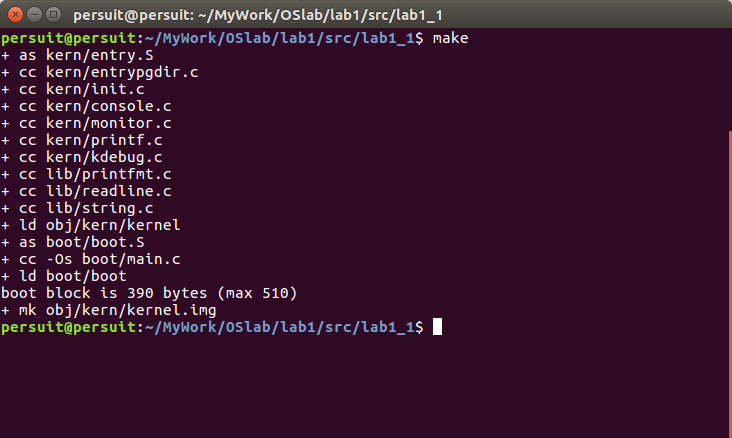
\includegraphics[scale=0.9]{figure/simu.png}
%		
%		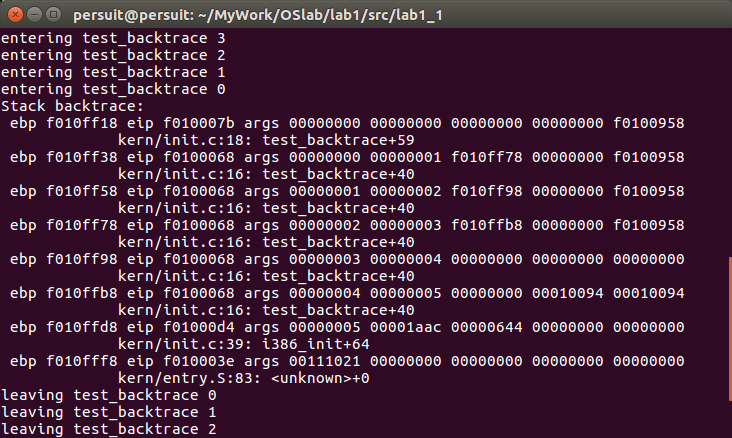
\includegraphics[scale=0.6]{figure/succ.png}
%		\caption X86模拟器安装成功
%	\end{figure}
%\section{BIOS}
%cd到lab1目录下,运行make qemu-gdb,另打开一个终端,运行gdb,我们能可以看到如图1.2信息
%	\begin{figure}[htbp!]
%		\centering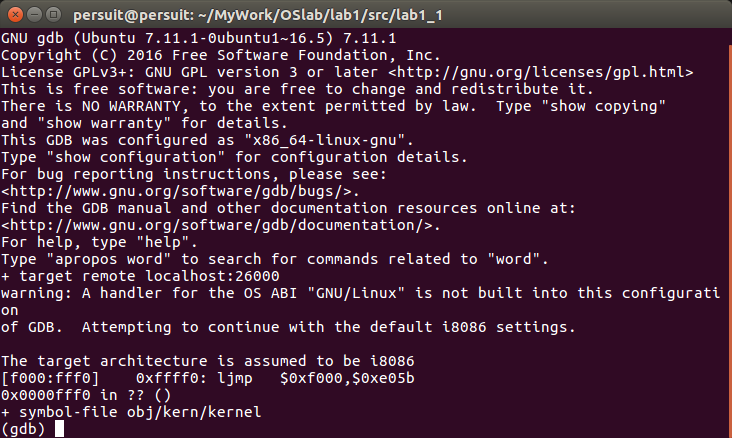
\includegraphics[scale=0.6]{figure/BIOS}
%		\caption{成功进入BIOS并执行第一个命令jmp}
%	\end{figure}
%\chapter{引导加载程序}
\chapter{PC Bootstrap}
\songti\zihao{-4}
\section{exercise 2}
使用GDB的si指令,我们跟踪了ROM BIOS 的前八条指令,如图1.1所示。接下来我们简单分析以下这八条指令的意义。
\begin{figure}[htbp!]
	\centering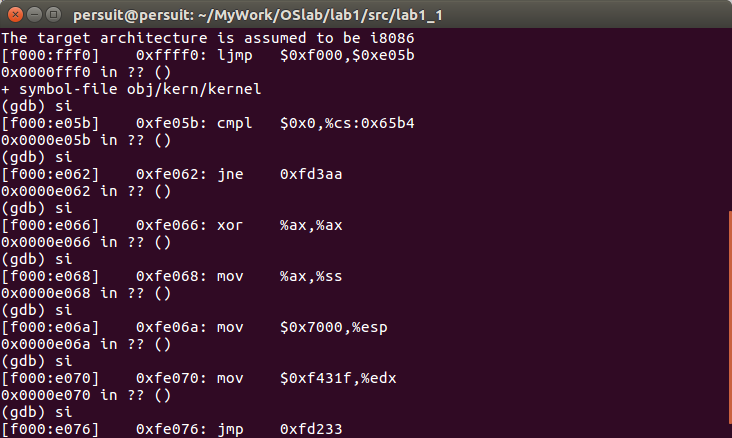
\includegraphics[scale=0.5]{figure/exercise2}
	\caption{ROM BIOS 的前八条指令}
\end{figure}
\begin{lstlisting}[language={[x86masm]Assembler}]
1. 0xffff0: ljmp $0xf000,$0xe05b
\end{lstlisting}
第一条命令是一个跳转指令,跳转到0xfe05b,地址推断方法为断寄存器值左移四位,然后和段内地址相加。

\begin{lstlisting}[language={[x86masm]Assembler}]
2. 0xfe05b: cmpl $0x0, $cs:0x6ac8
\end{lstlisting}
cmpl指令:将立即数0x0与\$cs:0x6ac8所代表的内存地址的值进行比较。cs为代码段寄存器
\begin{lstlisting}
3. 0xfe062:  jne  0xfd2e1
\end{lstlisting}
jne指令:如果ZF标志位不为0时跳转的0xfd2e1,即上一条指令中两者数值不等时跳转。
\begin{lstlisting}
4. 0xfe066:  xor  %dx, %dx
\end{lstlisting}
xor指令:异或位运算,相同位不同为1,相同为0,此条指令实际在清零dx寄存器
\begin{lstlisting}
5. 0xfe068:  mov  %dx %ss
6. 0xfe06a:  mov  $0x7000, %esp
7. 0xfe070:  mov  $0xf34d2, %edx
8. 0xfe076:  jmp  0xfd15c
\end{lstlisting}
上述指令同样是在做一些寄存器的赋值以及地址的跳转\\[0.3cm]

通过继续对指令的分析,我们可以看出正如实验指导上所说的,BIOS主要是在做一些初始化的,检测硬件设备,以及最重要的加载bootloader等。

\chapter{The Boot Loader}
\section{exercise 3}
按照实验要求,在追踪阅读了boot/boot.S,并结合obj/boot/boot.asm 及相关代码后,我们接下来回答以下问题。

\textcolor{red}{1.处理器什么时候开始执行32位代码?如何完成从16位到32位模式的切换?}\par
答:在运行 ljmp \$PROT\_MODE\_CSEG, \$protcseg 指令后,开始执行32bit代码。在boot.S中,PC首先处于real mode,以.code16即16bit运行,在real model 使能高于20的地址线,完成real mode到protected mode,从而完成.code16到.code32 的转化。可参考boot.S中的代码及注释。\par

\begin{figure}[htbp!]
	\centering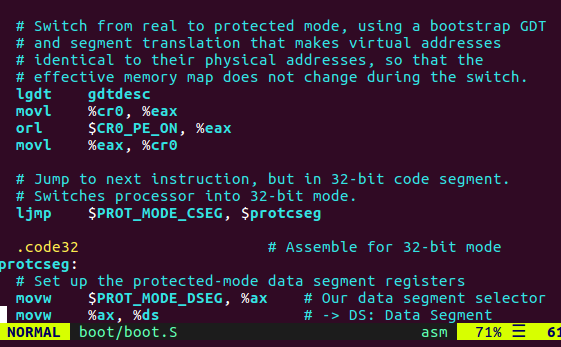
\includegraphics[scale=0.5]{figure/real2pro}
	\caption{boot.S中由16bit跳转到32bit的部分代码}
\end{figure}
\textcolor{red}{2.引导加载程序bootloader执行的最后一个指令是什么?加载的内核第一个指令是什么?}\par
答:bootloader由boot/boot.S和main.c组成。追踪到最后一个指令:
\begin{lstlisting}
	((void (*)(void)) (ELFHDR->e_entry))();
\end{lstlisting}\par
加载的内核的第一个指令在kern/entry.S:
\begin{lstlisting}
	movw    $0x1234,0x472           # warm boot
\end{lstlisting}

\textcolor{red}{3.内核的第一个指令在哪里?}\par
答:kern/entry.S\par
\textcolor{red}{4.引导加载程序如何决定为了从磁盘获取真个内核读取多少扇区?在哪里可以找到这些俄信息?}\par
答:在Program Header Table中的每一个表项分别对应操作系统的段,内容包括段的大小,段起始地址偏移等信息,由此表我们可以确定内核占用多少扇区。其中表存放在操作系统内核映像的ELF头部信息中。

\section{exercise 4}
\textcolor{red}{通读K&R书中5.1(指针和地址)到5.5(字符指针和函数)的内容。然后下载pointers.c的代码,运行它,并确保你了解所有打印值的来源。特别是,请确保你理解第1行和第6行中指针指向哪里的地址,第2行到第4行的值是如何被写入的,以及为什么第5行中打印的值看起来像是错乱的。}

答:如下图为pointers.c的运行结果。我们主要来看一下第1,5,6行的显示。\\
\textbf{首先来看第1行的三个地址:}\par
a:输出的是数组a的首地址,是在程序的栈中分配的。\par
b:输出的是指针b所指向的由操作系统在堆中分配的空间的起始地址。\par
c:输出的是未定义的指针变量的值\\
\textbf{接下来看第5行的显示:}\par
a[1]看起来乱码的原因是这句命令:c = (int *) ((char *) c + 1);这条语句把int*强制转化为char*并加1然后在强制转化为int*,0xbfb4bf89~0xbfb4bf8c,不再等于(a+1):0xbfb4bf88~0xbfb4bf8b,所以会出现类似"乱码"现象。\\
\textbf{最后第6行的显示参考以上分析。}\\

\begin{figure}[htbp!]
	\centering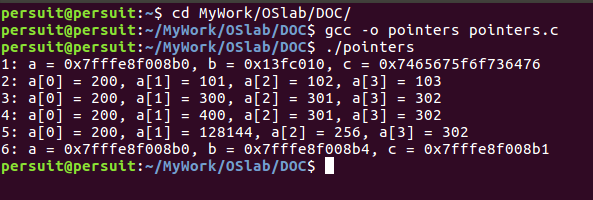
\includegraphics[scale=0.8]{figure/pointers}
	\caption{编译并运行pointers.c的结果}
\end{figure}

\section{exercise 5}
\textcolor{red}{跟踪bootloader程序的前几个指令,找到开始使用链接地址的第一条指令,即,如果你使用了错误的链接地址,那么执行到这里的时候就必须要停下来,否则就会发生错误。然后将boot/Makefrag中的链接地址更改为一个错误的地址,运行make clean,用make命令重新编译实验,然后再次跟踪到引导加载程序,看看会发生什么。不要忘了改变链接地址后要再次执行make clean!}\par
答:有前边所讲,链接地址即通过编译器链接器处理形成的可执行程序中指令的地址,加载地址是可执行文件真正被装入内存后运行的地址。在bootloader运行时仍处于实模式,此时链接地址等于加载地址。根据题目要求,我们要改动bootloader的链接地址0xc7c00.重新make,比较前后的obj/boot/boot.asm,如下图:可见两者的链接地址不同。\par
\begin{figure}[htbp]
	\centering
	%\includegraphics[scale=0.4]{figure/asm}
	\subfigure[更改链接地址前的boot.asm]{
	\begin{minipage}{7cm}
		\centering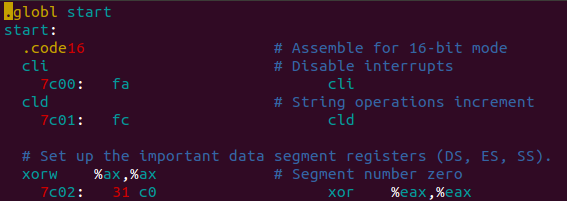
\includegraphics[scale=0.6]{figure/asm-old}
	\end{minipage}
	}
	\subfigure[更改链接地址后的boot.asm]{
		\begin{minipage}{7cm}
			\centering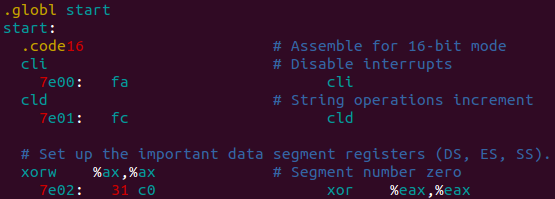
\includegraphics[scale=0.6]{figure/asm-new}
		\end{minipage}
		}
\end{figure}
考虑到BIOS默认把bootlader装入0x7c00处,当我们再次设置断点在0x7c00时,继续用si单步调试,发现在加载全局描述表寄存器GDTR时出现如图错误。显然GDTR的值不应该为0。

\section{exercise 6}
\textcolor{red}{复位机器(退出QEMU / GDB并再次启动)。在BIOS进入引导加载程序的那一刻停下来,检查内存中0x00100000地址开始的8个字的内容,然后再次运行,到bootloader进入内核的那一点再停下来,再次打印内存0x00100000的内容。为什么这8个字的内容会有所不同?第二次停下来的时候,打印出来的内容是什么?(你不需要使用QEMU来回答这个问题,思考即可)}

答:在进入bootloader前,0x00100000内容发全为0。在进入内核时,此时bootloader已经将内核的各个程序段送入内存地址0x00100000,所以现在存放的就是内核的某一段的内容。

\chapter{Kernel}
\section{exercise 7}
\textcolor{red}{使用QEMU和GDB跟踪到JOS内核并停止在movl\%eax,\%cr0。 查看内存中在地址0x00100000和0xf0100000处的内容。 下面,使用GDB命令stepi单步执行该指令。 指令执行后,再次检查0x00100000和0xf0100000的内存。 确保你明白刚刚发生的事情。新映射建立后的第一条指令是什么,如果映射配置错误,它还能不能正常工作? 注释掉kern/entry.S中的movl\%eax,\%cr0,再次追踪到它,看看你的理解是否正确.}

答:由之前的学习得到entry的入口地址0x10000c,在运行movl\%eax,\%cr0之前,0x001000000和0xf0100000处的内容如下图,可见采用分页管理后,0xf0100000处的内容已经映射到0x100000

\begin{figure}[htbp!]
	\centering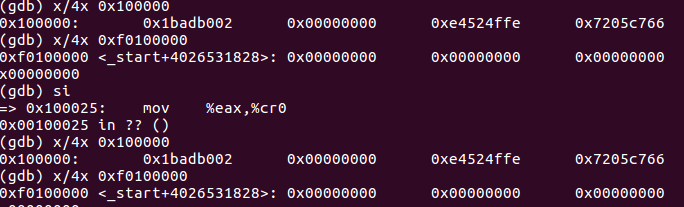
\includegraphics[scale=0.7]{figure/cr0}
	\caption{turn on page前后0xf0100000处的内容对比}
\end{figure}

\section{exercise 8}
	\textcolor{red}{阅读kern/printf.c,lib/printfmt.c和kern/console.c,并确保你了解他们的关系。我们省略了一小段代码,使用“\%o”形式的模式打印八进制数字所需的代码。查找并补全此代码片段}
	
	kern/printf.c是最高层的调用,其中cprintf调用了lib/printfmt.c中的vprintfmt子程序,putch调用了kern/console.c的cputchar子程序。前者在调整输出格式,主要是int。而console.c则主要为之完成CGA的单个字符显示,同时提供‘High'-level console I/O接口。
	
	\textcolor{red}{解释一下console.c文件中,下面这段代码的含义}
	\begin{lstlisting}
if (crt_pos >= CRT_SIZE) {
    int i;
    memcpy(crt_buf, crt_buf + CRT_COLS, (CRT_SIZE - CRT_COLS) * sizeof(uint16_t));
    for (i = CRT_SIZE - CRT_COLS; i < CRT_SIZE; i++)
        crt_buf[i] = 0x0700 | ' ';
    crt_pos -= CRT_COLS;
    }
	\end{lstlisting}
	
	在console.c的注释中我们知道,采用的是Text-mode CGA/VGA display output。上网查阅相关资料,80*25的text-mode就是每页最多可显示80*25个字符,当我们要显示某个字符,我们需要指定显示的字符,位置给CGA。所以本段代码是在处理当前显示位置超过CRT\_SIZE即80*25的情况,memcpy将1-79行的内容复制到0-78行,for循环则是将79行置为空格,然后更新crt\_pos的位置。
	
	\textcolor{red}{跟踪以下代码并单步执行:}
	\begin{lstlisting}
	int x = 1, y = 3, z = 4;
	cprintf("x %d, y %x, z %d\n", x, y, z);
	\end{lstlisting}
	\textcolor{red}{回答下列问题:}
	\begin{itemize}
		\item \textcolor{red}{再调用cprintf()时,fmt是什么意思,ap是什么意思?}
		\item \textcolor{red}{按照执行的顺序列出所有对cons\_putc, va\_arg,和vcprintf的调用。对于cons\_putc,列出它所有的输入参数。对于va\_arg列出ap在执行完这个函数后的和执行之前的变化。对于vcprintf列出它的两个输入参数的值。}
	\end{itemize}
	答:fmt即 指向格式显示字符串的指针。ap是指向参数列表的字符型指针变量。\\
	调用顺序:
	\begin{lstlisting}
-->vcprintf("x \%d, y \%x, z \%d\n",[1,2,3])
-->cons\_putc('x')
-->va\_arg():ap=ap+sizeof(int)
-->con\_putc(1)

-->cons\_putc('y')
-->va\_arg():ap=ap+sizeof(int)
-->con\_putc(3)

-->cons\_putc('z')
-->va\_arg():ap=ap+sizeof(int)
-->con\_putc(4)

	\end{lstlisting}
	
	\textcolor{red}{运行下面的代码}
	\begin{lstlisting}
	unsigned int i = 0x00646c72;
	cprintf("H%x Wo%s", 57616, &i);
	\end{lstlisting}
	\par
	输出:\raisebox{-1mm}{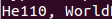
\includegraphics[scale=1]{figure/hello}},原因\%x是按照16进制输出57616显示为e110.int i分配四个字节,按照小端存储,四个字节分别存储0x72('r'),0x6c('l'),0x64('d'),0x03('\textbackslash0'),cprintf按照i的内存地址开始逐字节遍历并显示,正好输出"world"。
	
	\textcolor{red}{看下面代码,y=后会出现什么,为什么?}
	\begin{lstlisting}
    cprintf("x=%d y=%d", 3);
	\end{lstlisting}
	结果为: \raisebox{-1mm}{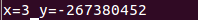
\includegraphics[scale=1]{figure/y}},由于y并没有参数被指定,所以会输出一个不确定的值。
	
	\textcolor{red}{假设GCC更改了它的调用约定,以声明的顺序将参数压入栈中,这样会使最后一个参数最后被压入。 你将如何更改cprintf或其接口,以便仍然可以传递一个可变数量的参数?}\\
	第一个想法是修改va\_list 变量,增加一个指向最后一个变量的指针。va\_arg实现由栈顶到栈抵的访问。\\
	
	
	\textcolor{red}{挑战 增强控制台的能力以允许以打印不同颜色的文本。传统的方法是使它解析嵌入在待打印的文本字符串中的ANSI转义序列,但是你可以使用任何你喜欢的机制。 在实验的参考内容和网络上其他地方有对VGA显示硬件进行编程的大量信息。 如果你真的喜欢挑战,也可以尝试将VGA硬件切换到图形模式,并使控制台将文本绘制到图形帧缓冲区上}
	
\section{exercise 9}
\textcolor{red}{确定内核在哪里完成了栈的初始化,以及栈所在内存的确切位置。内核如何为栈保留空间?栈指针初始化时指向的是保留区域的“哪一端”}
	
答:在entry.S中我们可以看到执行了 movl \$0x0,\%ebp 和 movl \$(bootstacktop),\%esp时已经处于虚拟地址。通过反汇编我们得到bootstacktop值为0xf0110000,在定义bootstacktop之前,分配了KSTKSIZE=8*PGSIZE=8*4kB=32kB,所以bootstack分配的空间为0xf0108000-0xf0110000,对应物理内存为0x108000-0x110000。

\textcolor{red}{内核如何给堆栈保留内存空间}\\
如上分析,在entry.S的数据段声明了大小为32kB的空间作为堆栈使用,从而为内核保留一块空间。

\textcolor{red}{堆栈指针又是指向这块被保留的区域的哪一端的呢?}

因为堆栈是向下的,堆栈指针指向最高地址即bootstacktop。

\textcolor{red}{要熟悉x86上C语言函数的调用约定,请在obj/kern/kernel.asm中找到test\_backtrace函数的地址,在其中设置一个断点,并检查在内核启动后每次这个函数被调用时会发生什么。 每一级的test\_backtrace在递归调用时,会在栈上压入多少个32位的字,这些字的内容是什么?}

会压入4个32位的字包括:返回地址,调用者的ebp,寄存器ebx,传递参数
	
\section{exercise 11}
\textcolor{red}{实现如上所述的回溯功能。 请使用与示例中相同的格式,否则打分脚本将会出错。当你认为你的工作正确的时候,运行make grade来看看它的输出是否符合我们的打分脚本所期待的,如果没有,修正发现的错误。在你成功提交实验1的作业后,欢迎你以任何你喜欢的方式更改回溯功能的输出格式。}

由exercise 10的分析可以得知函数在调用子函数对栈的操作\\
\begin{figure}[htpb!]
	\centering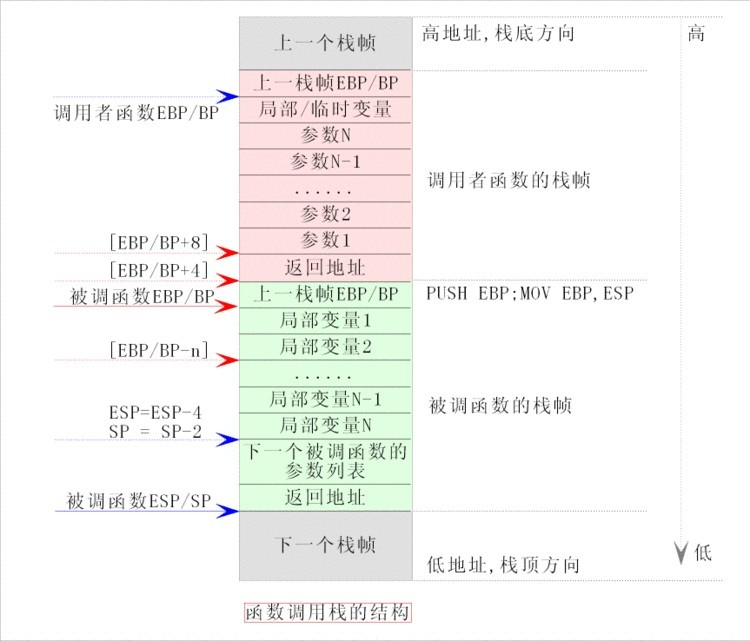
\includegraphics[scale=0.7]{figure/stack.jpg}
\end{figure}
结合反汇编代码:
\begin{figure}[htpb!]
	\centering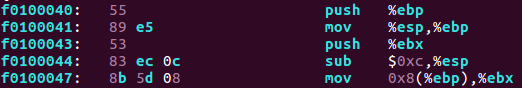
\includegraphics[scale=0.7]{figure/backtrace}
	\caption{调用testbaktrace子函数的部分反汇编代码}
\end{figure}
易得本题code:
\begin{lstlisting}
    uint32_t *ebp=(uint32_t*)read_ebp();
    uint32_t eip=ebp[1];
    cprintf("Stack backtrace:\n");
    while(ebp){
        cprintf(" ebp %08x eip %08x args ",ebp,eip);
	    int i=2;
	    for (i;i<7;++i){
	        cprintf("%08x ",ebp[i]);
	    }
    ebp=(uint32_t*) ebp[0];
    eip=ebp[1];
	}
    cprintf("\n");
	
\end{lstlisting}

\section{exercise 12}
\textcolor{red}{修改你的堆栈回溯功能,为每个eip显示与该eip对应的函数名称,源文件名和行号}

这个问题没看懂,代码是copy网上的。

\end{document}          